\documentclass[a4paper,12pt]{article}
\usepackage{perso}
\begin{document}
\titlepages[%
	author = {Chaste Gauvain, Ooms Aurélien},%
	course = INFO-F-404 : Real-Time Operating Systems,%
	COURSE = INFO-F-404,%
	title = Project 1: Least Laxity First,%
	bg = bg/ulb,%
	logo = logo/ulb,%
	faculty = Faculty of Science,%
	department = Computer Science Dept.,%
	university = Université Libre de Bruxelles,%
	academicyear = Academic year 2013~-~2014%
]
\begin{abstract}
\pagestyle{empty}
Study of the performance of LLF scheduling algorithm on systems with periodic, synchronous tasks
and constrained deadlines.
We consider systems of n periodic, synchronous and independent tasks $\tau = \{\tau_1 , \tau_2 , \dots , \tau_n \}$
with constrained deadlines embedded on a uniprocessor device.
The work is divided in 3 parts: implementation of a LLF scheduling algorithm simulator, implementation of a system generator and study of LFF's performances.
\end{abstract}

\maketoc
\newpage\cleardoublepage\phantomsection
\section{Simulator}
\label{sec:sim}

We implemented two versions of the simulator, one time based and one event based.
\subsection{General structure}

\begin{figure}
	\centering
	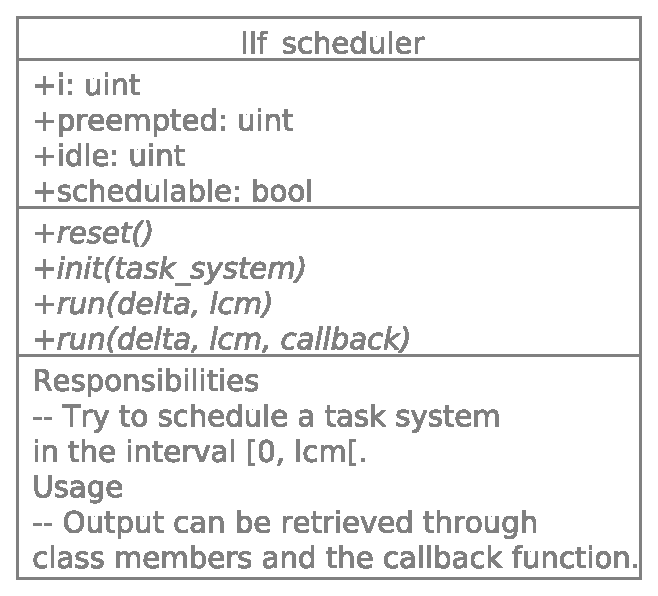
\includegraphics[width=0.5\textwidth]{fig/sim/1}
	\caption{\label{fig:sim:1} Interface of a scheduler}
\end{figure}

 \ref{fig:sim:1} describes the interface of both implementations. A use case can be seen in \ref{code:sim:1}.

\myinputminted[firstline=154,lastline=157]{c++}{../src/simLLF.cpp}{Use case of the scheduler interface}{code:sim:1}{3}

\nb{All the functionalities are splitted into small tools with aim to better flexibility, so for example in \ref{code:sim:1} you can see that the \emph{lowest common multiple} is computed outside of the scheduler.}
\subsection{Time based}

We first implemented the time based simulator for it's simplicity (\href{../h/os/llf_scheduler_time_based.h}{See file}).

A run of the scheduler looks like \ref{alg:sim:1}

\inputalgorithm[H]{Run of the time based scheduler}{alg:sim:1}{alg/sim/1}

Jobs are queued in an \emph{std::multimap<uint, os::job\_t>} where the key is the point in time where the job should imperatively be scheduled (start deadline) or else the system is not schedulable.
This is better (from the implementation point of view) than directly considering the slack time because the start deadline will only increment for the current job whereas slack times would decrement for all idle jobs (not optimal for priority queues).

$\Delta_r$ has been interpreted as : \emph{priorities of jobs are checked with a frequency of $\frac{1}{\Delta_r}$. However, if a job finishes, the cpu is left free and a new job can be handled without regards to $\Delta_r$.}
\subsection{Event based}

The event based scheduler can be easily obtained by modifying the time based scheduler, the only changes to make are:
\begin{enumerate}
	\item adding an event priority queue
	\item adding triggers for events
	\item computing the $i$ steps as $i = hpe.i$ where $hpe$ is the \emph{highest priority event}
\end{enumerate}

An example of the differences of implementations can be seen in \ref{code:app:1} and \ref{code:app:2}.

The event loop can be seen in \ref{code:app:3}.


(\href{../h/os/llf_scheduler_event_based.h}{Link to the source code}.)
\subsection{Time vs Event}

There are pros and cons considering both implementations. Here are listed some observations:

\begin{enumerate}
	\item The event based approach consumes more memory because of the (small) overhead of the event queue.
	\item The event based approach is much faster for $\Delta_r > 1$ (asymptotic $\Delta_r$ speed up factor).
	\item The time based approach has to check very often if new jobs appeared. This is very inconvenient in the case of long long period tasks (1 check per time unit).
\end{enumerate}

\newpage\cleardoublepage\phantomsection
\section{Task System Generator}
\label{sec:gen}
\subsection{Uniform distribution}

\subsubsection{Random partitioning}

We focused on producing uniformely distributed utilizations.

Suppose we want to generate a system $\tau = \{\tau_1 , \tau_2 , \dots , \tau_n \}$ with

\begin{equation}
	C_i \geq 1 \qquad \forall 1 \leq i \leq n
	\label{eq:WCET minimum}
\end{equation}

\begin{equation}
	\sum_{i=1}^{n} U_i + \epsilon = U
	\label{eq:Usage shift}
\end{equation}

\begin{equation}
	\text{minimize}~\epsilon
	\label{eq:Economic function of the generator}
\end{equation}

\begin{equation}
	\epsilon \geq 0
	\label{eq:Usage shift polarity}
\end{equation}

We choose $n-1$ partition $p_j \in P = ~]0, U[$ with

\begin{equation}
	|p_j - p_k| \geq \frac{1}{T_{min}} \qquad \forall p_j \in P, p_k \in P \cup \{0, U\}, p_j \neq p_k
	\label{eq:Discrete partition condition}
\end{equation}

To achieve \ref{eq:Discrete partition condition} we define the \emph{floor\_min\_uniform} function (see \ref{code:gen:1}).

\myinputminted[firstline=10,lastline=17]{c++}{../h/os/generator.h}{The \emph{floor\_min\_uniform} function}{code:gen:1}{1}

An example of use can be seen in \ref{code:app:4}.

(\href{../h/os/generator.h}{Link to the source code}.)

\subsubsection{Limits}

The \emph{lowest common multiple} is exponential in $n$. If we only use the primitive types provided by the \CXX~language we are bounded to a \emph{max} value.

Sufficient condition for the feasability of lcm computation

\begin{equation}
	T_{max}^n \leq 2^b-1
	\label{eq:Lowest common multiple condition}
\end{equation}

Where
\begin{conditions}
	T_{max}		&	the maximum value of the period distribution\\
	n			&	number of tasks in the system \\
	2^b-1		&	the maximum value for an integer
\end{conditions}

Another requirement was to never overflow the $U$ asked by the user.

Sufficient condition for a non-overflowing total usage

\begin{equation}
	U_i \geq \frac{1}{T_i}
	\label{eq:Usage no-overflow warranty}
\end{equation}

Where
\begin{conditions}
	U_i	&	usage of $\tau_i$ \\
	T_i	&	period of $\tau_i$
\end{conditions}

For \ref{eq:Economic function of the generator} we can note that

\begin{equation}
	\epsilon_{max} = \frac{n}{T_{max}}
	\label{eq:Usage shift maximum}
\end{equation}

We decided not to attach much importance to \ref{eq:Economic function of the generator} because of the spectrum of study considered (see \ref{sec:study}).
\subsection{Specific Populations}

In the previous section we exposed the way we chose to produce a uniform distribution of task systems.

This implementation will be used in \ref{sec:study} but we could ask ourselves if there is no other option.
It would be interesting to be able to study a specific population of task systems, this could be achieved with discrete non-uniform distributions of individual tasks.
\newpage\cleardoublepage\phantomsection
\section{Study}
\label{sec:study}
\subsection{Spectrum}

We studied the following ranges of values
\begin{itemize}
	\item{$U$} [0.1, 0.2, 0.3, 0.4, 0.5, 0.6, 0.7, 0.8, 0.9, 1]
	\item{$\Delta_r$} [1, 2, 3, 4, 5, 6, 7, 8, 9, 10]
	\item{$n$} [2, 3, 4]
	\item{$k$} 1000
	\item{$T_{min}$} 50
	\item{$T_{max}$} 100
\end{itemize}

The systems are generated with the technique explained in \ref{sec:gen}.

Reading \ref{eq:Usage no-overflow warranty} we have the warranty that $\epsilon_{max} = \frac{n}{T_{min}} \leq 0.08 < 0.1$.
We can thus consider that results for $U$ will be a biased mean of values in the interval $[U-0.08, U]$.

We choose $n$ and $T_{max}$ small because of \ref{eq:Lowest common multiple condition}.


\nb{A system is generated for each triple $(U, n, k)$, this system is tested against the range of $\Delta_r$ values.}
\subsection{Results}

\nb{The preemption rate is computed as $\frac{scheduler.preempted}{lcm}$ if the system is schedulable with the current configuration, $\frac{scheduler.preempted}{scheduler.i}$ otherwise (for schedulable systems $lcm = scheduler.i$).}


\ref{fig:stu:au} shows an exponential decrease of the schedulability rate in $u$ as well as a nearly linear increase of preemption rate with constant factor $0.1$.

\begin{figure}
	\centering
	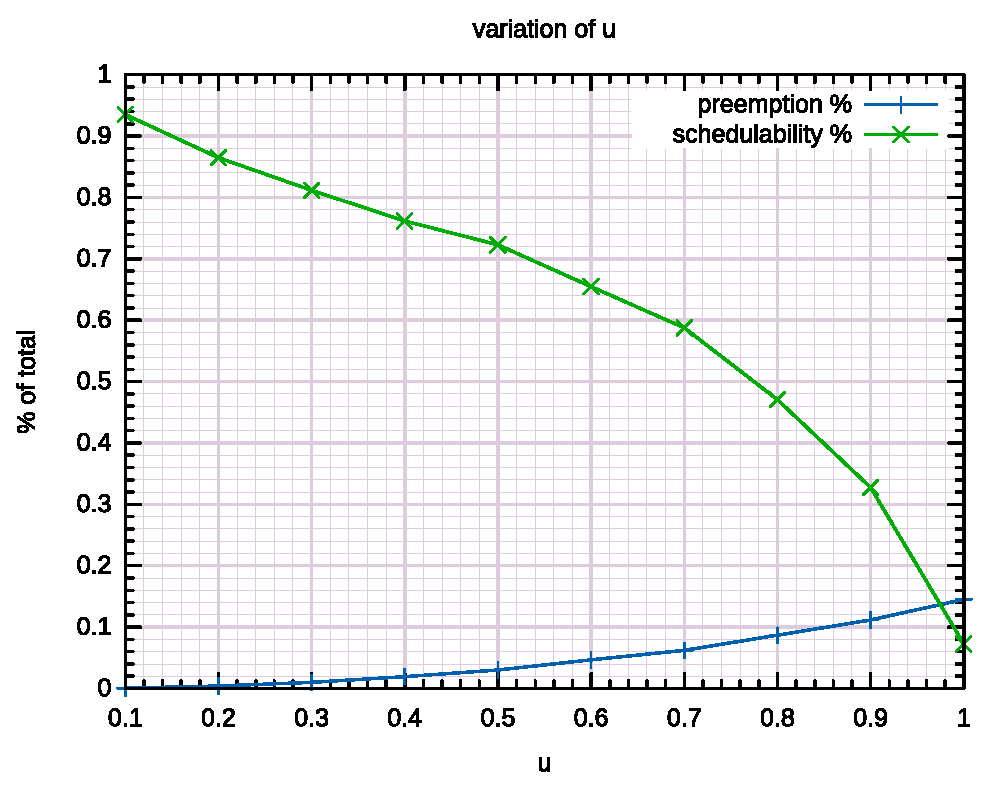
\includegraphics[width=0.8\textwidth]{../gnuplot/eps/1}
	\caption{\label{fig:stu:au} Schedulability and preemption rate depending on $u$}
\end{figure}


\ref{fig:stu:ad} shows a nearly linear decrease of the schedulability rate in $\Delta_r$ with constant factor $0.02$ as well as a negative exponential decrease of the preemption rate.

\begin{figure}
	\centering
	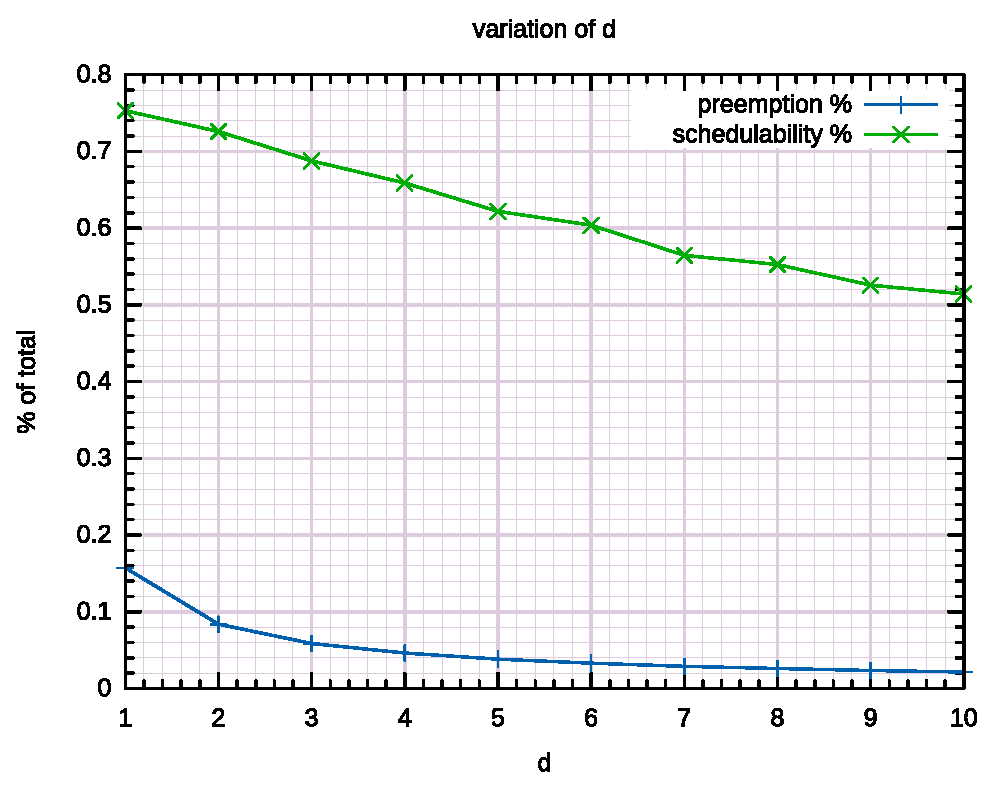
\includegraphics[width=0.8\textwidth]{../gnuplot/eps/2}
	\caption{\label{fig:stu:ad} Schedulability and preemption rate depending on $\Delta_r$}
\end{figure}

\ref{fig:stu:an} shows a nearly linear decrease of the schedulability rate in $n$ as well as a linear increase of the preemption rate. This result is probably not exploitable since the range of $n$ value is not wide enough.

\begin{figure}
	\centering
	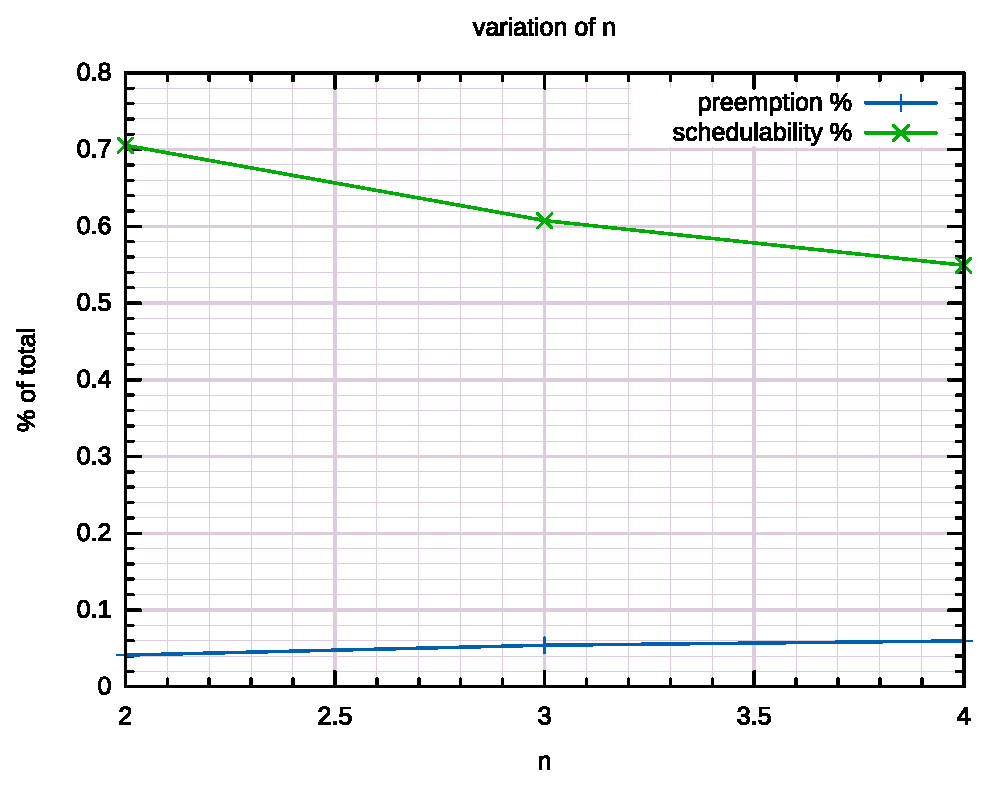
\includegraphics[width=0.8\textwidth]{../gnuplot/eps/3}
	\caption{\label{fig:stu:an} Schedulability and preemption rate depending on $n$}
\end{figure}

\ref{fig:stu:4p} shows the influence of $u$ and $\Delta_r$ on the preemption rate ($n = 4$).

\begin{figure}
	\centering
	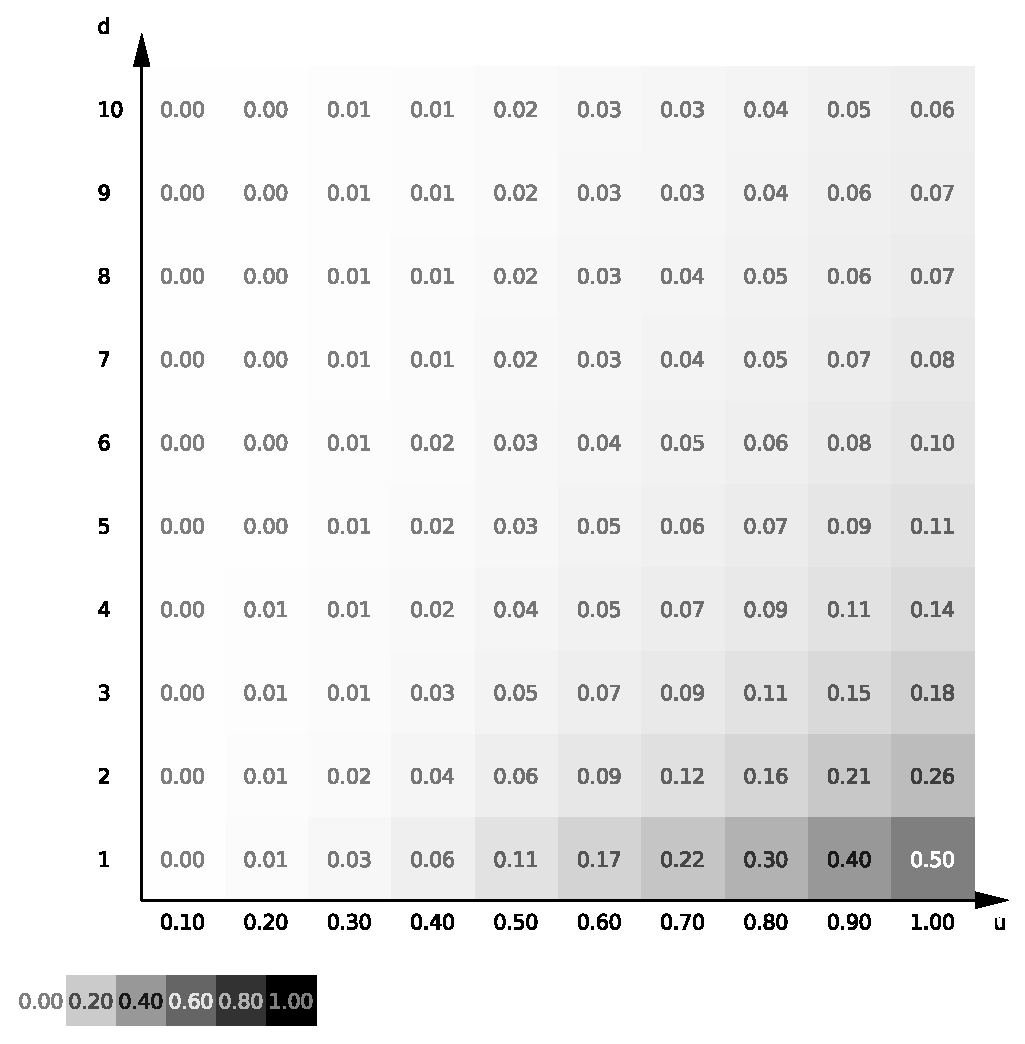
\includegraphics[width=1\textwidth]{../mean/eps/4p}
	\caption{\label{fig:stu:4p} Preemption rate for $n = 4$}
\end{figure}

\ref{fig:stu:4s} shows the influence of $u$ and $\Delta_r$ on the schedulability rate ($n = 4$).

\begin{figure}
	\centering
	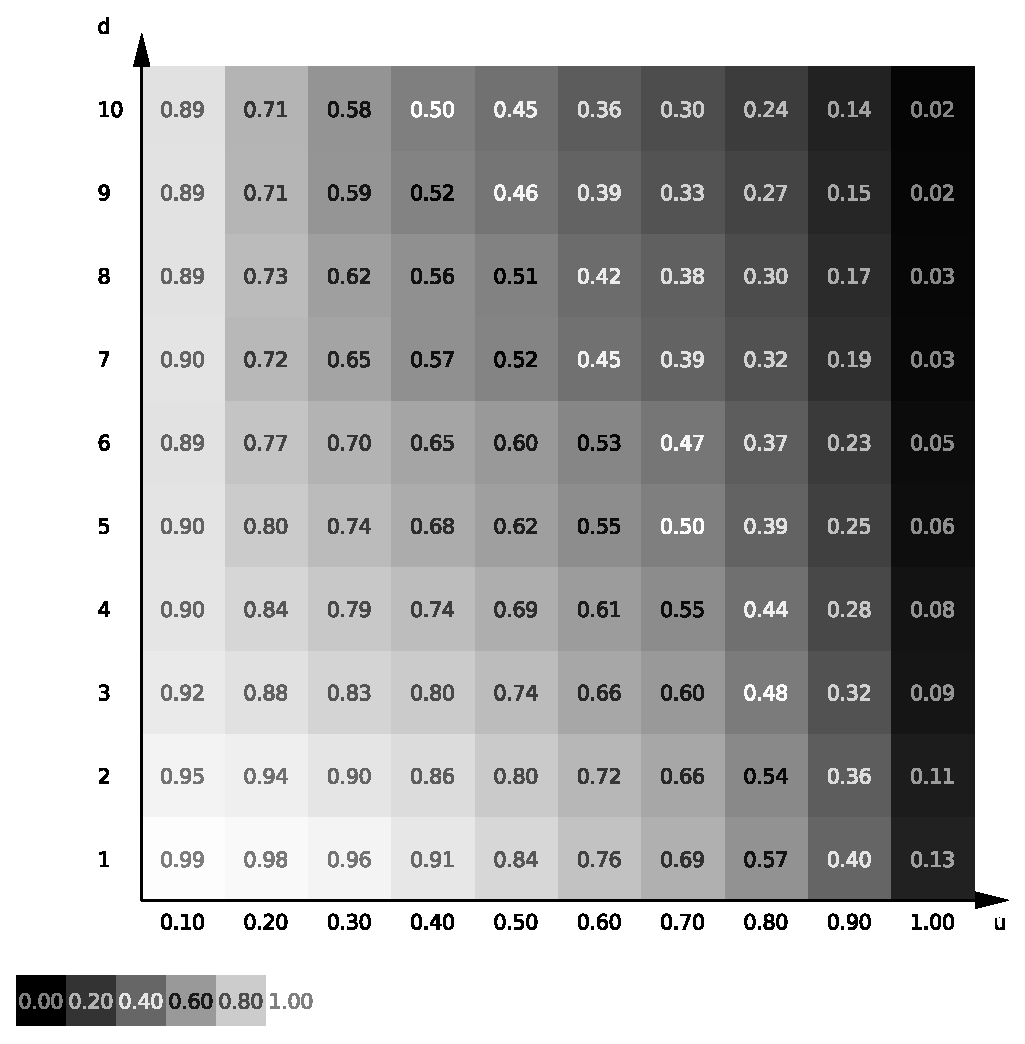
\includegraphics[width=1\textwidth]{../mean/eps/4s}
	\caption{\label{fig:stu:4s} Schedulability rate for $n = 4$}
\end{figure}

\subsection{Interpretation}

The results are not surprising.

\begin{conditions}
	$S$ & schedulability rate\\
	$P$ & preemption rate
\end{conditions}

\begin{equation}
	\uparrow U \Rightarrow ~\downarrow S ~~\land ~\uparrow P
	\label{eq:U influence}
\end{equation}

\begin{equation}
	\uparrow \Delta_r \Rightarrow ~\downarrow S ~~\land ~\downarrow P
	\label{eq:d influence}
\end{equation}

\begin{equation}
	\uparrow n \Rightarrow ~\downarrow S ~~\land ~\uparrow P
	\label{eq:n influence}
\end{equation}


The exponential decrease of the schedulability rate in $u$ shown in \ref{fig:stu:au} suggests that
to achieve a good use of the whole computation capabilities of the cpu some engineering to design the task system has to be done.
\newpage\cleardoublepage\phantomsection
\section{Use Cases}
\label{sec:use}
\subsection{Simulator}


\subsubsection{Regular mode}

\shellcmd{./run/simLLF 10 system/1}

\shellcmd{cat system/1 | ./run/simLLF 10}


\subsubsection{Event pipe mode}

\shellcmd{cat system/3 | ./run/simLLF 10 -p | ./run/plot\_schedule shedule/svg/1.svg -g 10}

\ref{fig:use:1} shows the output of this command.

\begin{figure}
	\centering
	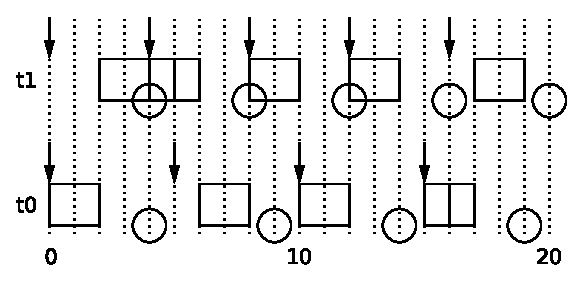
\includegraphics[width=0.9\textwidth]{../schedule/eps/1.eps}
	\caption{Output of the event pipe mode}
	\label{fig:use:1}
\end{figure}

\subsection{Generator}

\shellcmd{./run/taskGenerator -u 0.7 -n 4}

You can use the \verb#--verbose# option to see more information.

You can use the \verb#--seed# option to choose the seed of the generator.
\subsection{Study}


\subsubsection{Command line used for \ref{sec:study}}

\shellcmd{./run/LLF\_study -u 0.1 0.2 0.3 0.4 0.5 0.6 0.7 0.8 0.9 1 -d 1 2 3 4 5 6 7 8 9 10 -n 2 3 4 -k 1000 > benchmark/1}



\subsubsection{Splitting data for \emph{gnuplot}}

\shellcmd{cat benchmark/1 | ./run/gnuplot -o gnuplot/data/1 gnuplot/data/2 gnuplot/data/3}



\subsubsection{Plot data with \emph{gnuplot}}

\shellcmd{./tools/gnuplot/render u gnuplot/data/1 gnuplot/svg/1.svg}

\shellcmd{./tools/gnuplot/render d gnuplot/data/2 gnuplot/svg/2.svg}

\shellcmd{./tools/gnuplot/render n gnuplot/data/3 gnuplot/svg/3.svg}



\subsubsection{Splitting data for custom color plot}

\shellcmd{cat benchmark/1 | ./run/split\_benchmark -o benchmark/2 benchmark/3 benchmark/4}

\shellcmd{cat benchmark/2 | ./run/compute\_mean -o mean/data/2p mean/data/2s}

\shellcmd{cat benchmark/3 | ./run/compute\_mean -o mean/data/3p mean/data/3s}

\shellcmd{cat benchmark/4 | ./run/compute\_mean -o mean/data/4p mean/data/4s}



\subsubsection{Plot data with custom color plot}

\shellcmd{cat mean/data/2p | ./run/plot\_mean -o mean/svg/2p --color 255 255 255 0 0 0}

\shellcmd{cat mean/data/2s | ./run/plot\_mean -o mean/svg/2s --color 0 0 0 255 255 255}

\shellcmd{cat mean/data/3p | ./run/plot\_mean -o mean/svg/3p --color 255 255 255 0 0 0}

\shellcmd{cat mean/data/3s | ./run/plot\_mean -o mean/svg/3s --color 0 0 0 255 255 255}

\shellcmd{cat mean/data/4p | ./run/plot\_mean -o mean/svg/4p --color 255 255 255 0 0 0}

\shellcmd{cat mean/data/4s | ./run/plot\_mean -o mean/svg/4s --color 0 0 0 255 255 255}

\appendix
\newpage\cleardoublepage\phantomsection
\section{Code}

Here are listed some interesting parts of the source code.


\subsection{Differences of scheduler implementation}

In \ref{code:app:1} and \ref{code:app:2} you can see that simulation steps computation differs.

\myinputminted[firstline=70,lastline=95]{c++}{../h/os/llf_scheduler_time_based.h}{Job progress (time based)}{code:app:1}{4}
\myinputminted[firstline=141,lastline=169]{c++}{../h/os/llf_scheduler_event_based.h}{Job progress (event based)}{code:app:2}{4}


\subsection{Event loop}

In \ref{code:app:3} you can see the event loop that allows much better performances in the event based implementation.

\myinputminted[firstline=99,lastline=128]{c++}{../h/os/llf_scheduler_event_based.h}{Event loop}{code:app:3}{4}

\subsection{Random partitioning}

\ref{code:app:4} shows the loop that fills the set of partitions.

\myinputminted[firstline=24,lastline=26]{c++}{../h/os/generator.h}{Usage of the \emph{floor\_min\_uniform} function}{code:app:4}{3}
%\makebib{bib/1}
\makefig
\makeequ
\makeminted
%\makethm
\makealg
\makeind
\end{document}
